\documentclass[11pt,a4paper]{article}

% ---------- Paquetes ----------
\usepackage[utf8]{inputenc}
\usepackage[T1]{fontenc}
\usepackage[spanish,es-tabla,es-nodecimaldot]{babel}
\usepackage[margin=2.5cm]{geometry}
\usepackage{booktabs}
\usepackage{array}
\usepackage{caption}
\usepackage{enumitem}
\usepackage{xcolor}
\usepackage{titlesec}
\usepackage{fancyhdr}
\usepackage{graphicx}
\usepackage{float}
\usepackage[colorlinks=true,linkcolor=black,citecolor=black,urlcolor=blue!50!black]{hyperref}
\newcommand{\dt}{.\allowbreak}
\newcommand{\us}{\_\allowbreak}
\newcommand{\var}[1]{\texttt{#1}}

\setlength{\parskip}{0.45em}
\setlength{\parindent}{0pt}
\captionsetup{font=small,labelfont=bf}
\renewcommand{\tablename}{Tabla}
\renewcommand{\arraystretch}{0.95}
\graphicspath{{figuras/}}

\titleformat{\section}{\normalfont\Large\bfseries}{\thesection.}{0.6em}{}
\titleformat{\subsection}{\normalfont\large\bfseries}{\thesubsection}{0.6em}{}
\titlespacing*{\section}{0pt}{1.2em}{0.6em}

\pagestyle{fancy}
\fancyhf{}
\fancyhead[L]{\small Machine Learning II --- Proyecto Integrador}
\fancyhead[R]{\small Segunda Entrega}
\fancyfoot[C]{\small\thepage}
\renewcommand{\headrulewidth}{0.4pt}

% ---------- Datos del proyecto ----------
\newcommand{\tituloProyecto}{Predicción de deserción estudiantil en el Tecnológico de Monterrey mediante modelado avanzado de Machine Learning}
\newcommand{\nombreCurso}{Machine Learning II}
\newcommand{\nombreProfesor}{Wilmer Pineda}
\newcommand{\repo}{\url{https://github.com/miguel-camargo611/ML2-desercion-estudiantil}}

\begin{document}

% ================= PORTADA =================
\begin{titlepage}
\centering
\vspace*{1.5cm}
{\Large\bfseries Universidad Externado de Colombia\par}
\vspace{0.2cm}
{\large Departamento de Matemáticas\par}
\vspace{0.15cm}
{\large \nombreCurso\par}
\vspace{2.2cm}

{\large\scshape Proyecto Integrador --- Segunda Entrega\par}
\vspace{0.2cm}
{\normalsize Fase 2: datos, modelamiento y validación\par}
\vspace{0.4cm}
\rule{0.6\linewidth}{0.4pt}
\vspace{0.6cm}

{\Huge\bfseries \tituloProyecto \par}
\vspace{0.6cm}
\rule{0.6\linewidth}{0.4pt}

\vfill

\begin{minipage}{0.75\linewidth}
\centering
\textbf{Integrantes}\\[0.3cm]
Miguel Camargo \\
Camilo Hernández
\end{minipage}

\vspace{1.2cm}
\textbf{Profesor:} \nombreProfesor

\vspace{0.8cm}
\textbf{Código reproducible:} \repo

\vspace{1.2cm}
{\large 27 de septiembre de 2026 \par}
\vfill
\end{titlepage}

\pagenumbering{arabic}
\setcounter{page}{1}

% ================= INTRODUCCIÓN =================
Este informe presenta la segunda fase del proyecto: la consolidación de los datos, la construcción de un flujo de modelamiento sin fuga de información, la reproducción del método de Villar y Andrade (2024) y la evaluación de los modelos. El problema consiste en predecir qué estudiantes de pregrado abandonan la universidad durante su primer año, con el fin de ofrecerles acompañamiento a tiempo. El código y las instrucciones para reproducir cada resultado están en el repositorio indicado en la portada.

% ================= SECCIÓN 1 =================
\section{Consolidación de los datos}

\textbf{Fuente.} Se utilizó el \textit{Student Dropout Dataset} del Tecnológico de Monterrey (Alvarado-Uribe et al., 2022), obtenido mediante solicitud formal al IFE Data Hub. Contiene 143.326 registros de estudiantes de bachillerato y pregrado pertenecientes a siete cohortes de ingreso, identificadas como AD14 a AD20: la cohorte AD14 agrupa a quienes iniciaron sus estudios en el semestre agosto--diciembre de 2014, y así sucesivamente hasta 2020. Al tratarse de datos reales latinoamericanos con más de 5.000 registros, no fue necesario recurrir a simulación.

\textbf{Población y variable objetivo.} El análisis se restringió a los 77.517 estudiantes de pregrado, población comparable a la del artículo. La variable objetivo es binaria: toma el valor 1 si el estudiante ya no está matriculado al terminar su primer año (\var{retention} $=0$ en el dataset) y 0 si continúa. El artículo distingue tres desenlaces (graduado, matriculado con rezago y desertor), pero este dataset no registra la graduación, por lo que el problema se planteó como clasificación binaria. La deserción afecta al 8,8\,\% de los estudiantes y varía poco entre cohortes (Figura~\ref{fig:cohorte}). Esta proporción es mucho menor que la del artículo (32\,\%), lo que hace al problema más desbalanceado y condiciona la elección de métricas (Sección~4).

\begin{figure}[H]
\centering
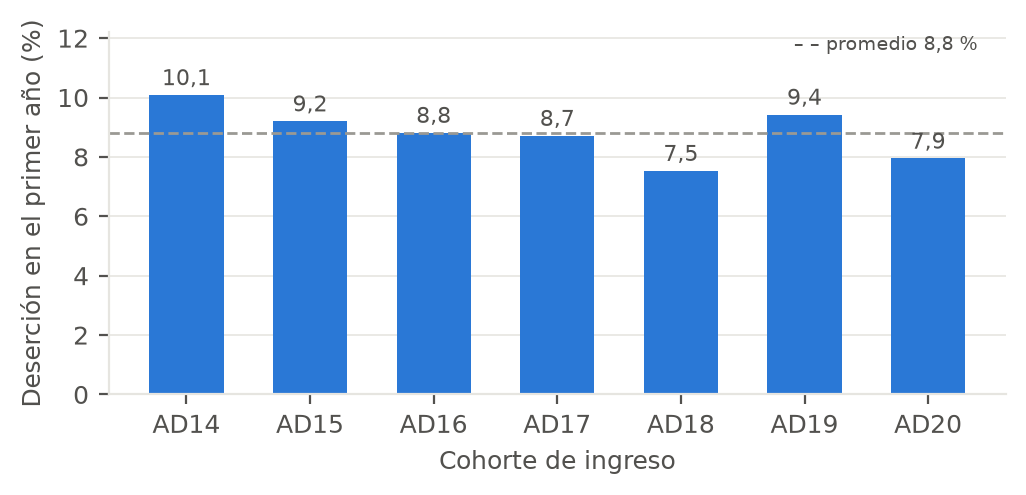
\includegraphics[width=0.62\linewidth]{fig01_desercion_cohorte.png}
\caption{Porcentaje de estudiantes de pregrado que desertan en su primer año, por cohorte de ingreso.}
\label{fig:cohorte}
\end{figure}

\textbf{Calidad de los datos.} La Tabla~\ref{tab:calidad} resume los problemas encontrados y la decisión adoptada en cada caso. El más importante es el de las actividades extracurriculares: el valor ``sin dato'' aparece sobre todo en estudiantes que desertaron, porque no alcanzaron a inscribirse en ellas. Usarlas le daría al modelo una pista que solo existe \emph{después} de la deserción.

\begin{table}[!t]
\centering
\footnotesize
\caption{Problemas de calidad encontrados y decisión adoptada.}
\label{tab:calidad}
\begin{tabular}{>{\raggedright\arraybackslash}p{5.4cm}>{\raggedright\arraybackslash}p{2.6cm}>{\raggedright\arraybackslash}p{6.2cm}}
\toprule
Problema & Magnitud & Decisión \\
\midrule
Variables socioeconómicas con el valor ``No information'' & 45--86\,\% de los registros & Se conserva ``sin dato'' como una categoría más, porque no ocurre al azar. \\
Puntajes de admisión faltantes (ingreso por otras vías) & 33--39\,\% & Se imputan con la mediana y se agrega una variable que indica que el dato faltaba. \\
Desempeño del primer semestre registrado solo en las cohortes AD19 y AD20 & 68\,\% sin dato & Se usa únicamente en el escenario B (ver abajo). \\
Estudiantes que aparecen más de una vez & 80 casos & La partición de los datos se hace por estudiante, no por registro. \\
Actividades extracurriculares cuyo ``sin dato'' corresponde en 75--84\,\% a desertores & 9 variables & Se excluyen: el dato falta porque el estudiante ya se había ido. \\
\bottomrule
\end{tabular}
\end{table}

\textbf{Variables utilizadas.} Además de las actividades extracurriculares, se excluyeron la variable que indica en qué semestre desertó el estudiante (solo es distinta de cero si ya desertó), la cohorte (un modelo en uso recibiría cohortes nuevas), el identificador, el colegio de origen (6.534 valores distintos) y cuatro variables duplicadas. No se crearon variables nuevas. Se conservaron 28 variables disponibles al momento del ingreso, agrupadas en cuatro bloques: \emph{demográficas} (edad, género, procedencia), \emph{socioeconómicas} (educación de los padres, nivel socioeconómico, becas y créditos), \emph{académicas de ingreso} (promedio de bachillerato, examen de admisión, nota de matemáticas, nivel de inglés) e \emph{institucionales} (campus, escuela, programa y carga académica).

\textbf{Dos momentos de predicción.} El artículo de Villar y Andrade mejora el trabajo previo de Martins et al. (2021) al añadir el desempeño académico de los primeros semestres a la información de ingreso. Para reproducir ese paso se definieron dos escenarios, que corresponden a dos momentos en los que la universidad podría hacer la predicción (Tabla~\ref{tab:escenarios}):
\begin{itemize}[leftmargin=1.2em,itemsep=1pt,topsep=2pt]
\item \textbf{Escenario A, al ingreso:} solo las 28 variables conocidas al matricularse. Incluye las siete cohortes.
\item \textbf{Escenario B, al terminar el primer semestre:} las 28 variables más tres de desempeño en ese semestre (promedio, materias reprobadas y materias retiradas). Como estas tres variables solo se registraron en AD19 y AD20, el escenario usa esas dos cohortes. Se excluye a quienes abandonaron \emph{durante} el primer semestre, porque su promedio refleja el abandono en lugar de anticiparlo.
\end{itemize}

\begin{table}[H]
\centering
\small
\caption{Tamaño de los conjuntos de datos. El conjunto de prueba se reserva para la entrega final.}
\label{tab:escenarios}
\begin{tabular}{lcrrrc}
\toprule
Escenario & Cohortes & Variables & Desarrollo & Prueba & Deserción \\
\midrule
A --- al ingreso & AD14--AD20 & 28 & 62.014 & 15.503 & 8,8\,\% \\
B --- al terminar el 1.\textsuperscript{er} semestre & AD19--AD20 & 31 & 19.408 & 4.843 & 7,8\,\% \\
\bottomrule
\end{tabular}
\end{table}

% ================= SECCIÓN 2 =================
\section{Flujo reproducible sin fuga de datos}

Hay \emph{fuga de datos} cuando el modelo usa, al entrenar, información que no tendría disponible al momento de predecir. El resultado son métricas optimistas que no se sostienen en la práctica. El flujo se diseñó con tres salvaguardas.

\textbf{1. Conjunto de prueba sellado.} Antes de cualquier modelamiento se separó el 20\,\% de los estudiantes como conjunto de prueba, que no se utilizará hasta la entrega final. La separación conserva la proporción de desertores y de cohortes, y asigna cada estudiante a un solo lado.

\textbf{2. Transformaciones dentro de un \texttt{Pipeline}.} Todas las transformaciones se encadenaron en un \texttt{Pipeline} en este orden: (1) imputación de los datos faltantes con la mediana; (2) estandarización de las variables numéricas; (3) codificación \textit{one-hot} de las variables categóricas; (4) sobremuestreo con SMOTE, que crea desertores sintéticos para equilibrar las clases, y (5) el clasificador. Cada paso calcula sus parámetros (medianas, medias, categorías y vecinos) solo con los datos de entrenamiento, y luego los aplica sin recalcularlos a los datos de validación. SMOTE se ejecuta únicamente al entrenar, de modo que la validación conserva la proporción real de desertores.

\textbf{3. Validación cruzada anidada.} Los datos de desarrollo se dividieron en cinco partes. En cada una de cinco rondas, cuatro partes se usan para entrenar y la quinta para evaluar. Dentro de las cuatro partes de entrenamiento, una segunda validación cruzada de tres partes elige los hiperparámetros y el umbral de decisión del modelo. Así, la parte usada para evaluar nunca interviene en ninguna elección. Los resultados se reportan como el promedio y la desviación estándar de las cinco rondas.

\textbf{Efecto de la fuga en el protocolo del artículo.} Villar y Andrade aplican SMOTE a todos los datos antes de separar entrenamiento y validación. Para medir el efecto de esa decisión se entrenó el mismo modelo (LightGBM, escenario A) con ambos protocolos (Tabla~\ref{tab:fuga}). Con el protocolo del artículo, los resultados parecen excelentes; con el flujo descrito, son modestos. La diferencia se explica porque, al aplicar SMOTE antes de separar, los desertores sintéticos de la validación son mezclas de estudiantes que el modelo ya vio al entrenar: el modelo reconoce casos casi repetidos en lugar de predecir casos nuevos. Esto sugiere que parte del alto desempeño reportado en el artículo (F1 de 0,83 a 0,88) proviene del protocolo y no del modelo.

\begin{table}[H]
\centering
\small
\caption{Mismo modelo evaluado con los dos protocolos (escenario A, 5 rondas). El PR-AUC se explica en la Sección~4.}
\label{tab:fuga}
\begin{tabular}{lcc}
\toprule
Protocolo & F1 deserción (umbral 0,5) & PR-AUC \\
\midrule
SMOTE antes de separar (artículo) & 0{,}94 & 0{,}98 \\
SMOTE solo en entrenamiento (este trabajo) & 0{,}03 & 0{,}19 \\
\bottomrule
\end{tabular}

\end{table}

% ================= SECCIÓN 3 =================
\section{Reproducción y adaptación del método}

El método del artículo consiste en comparar árboles y ensambles clásicos con cuatro algoritmos de \textit{boosting}, equilibrar las clases con SMOTE, ajustar los hiperparámetros e interpretar el mejor modelo con SHAP. La Tabla~\ref{tab:adaptacion} resume qué se conservó y qué se modificó.

\begin{table}[H]
\centering
\footnotesize
\caption{Reproducción y adaptación del método de Villar y Andrade (2024).}
\label{tab:adaptacion}
\begin{tabular}{>{\raggedright\arraybackslash}p{2.5cm}>{\raggedright\arraybackslash}p{4.6cm}>{\raggedright\arraybackslash}p{7.1cm}}
\toprule
Elemento & Artículo & Este trabajo \\
\midrule
Variable objetivo & Tres clases: graduado, rezagado y desertor & Binaria: deserta o no en el primer año (el dataset no registra graduación) \\
Modelos & Árbol, Random Forest, SVM, Gradient Boosting, XGBoost, LightGBM, CatBoost & Los mismos, más regresión logística como referencia y una variante de CatBoost sin SMOTE \\
Balanceo de clases & SMOTE sobre todos los datos & SMOTE solo sobre los datos de entrenamiento \\
Hiperparámetros & Optuna & \texttt{GridSearchCV}, herramienta del curso, dentro de la validación anidada \\
Métrica principal & F1 ponderado & PR-AUC, \textit{recall} y precisión de la clase deserción \\
Interpretación & SHAP & SHAP, repetido en cada ronda para verificar su estabilidad \\
\bottomrule
\end{tabular}
\end{table}

\textbf{Modelos comparados.} Se compararon diez modelos: dos líneas base (un clasificador que siempre predice la clase mayoritaria y un árbol de decisión sin poda), la regresión logística como referencia del curso anterior y siete modelos avanzados: Random Forest, SVM con kernel RBF, Gradient Boosting, XGBoost, LightGBM, CatBoost y \emph{CatBoost nativo}. Este último es una adaptación propia: CatBoost puede recibir las variables categóricas sin codificarlas y, en lugar de usar SMOTE, compensa el desbalance dando más peso a los desertores durante el entrenamiento. Para manejar el volumen de datos, la SVM usa una aproximación del kernel (Nystroem) y Gradient Boosting usa su versión por histogramas.

\textbf{Ajuste de hiperparámetros.} Para cada modelo se definió una rejilla con los hiperparámetros que controlan su complejidad (Tabla~\ref{tab:hiper}). En cada una de las cinco rondas, \texttt{GridSearchCV} probó todas las combinaciones y eligió la de mayor PR-AUC en la validación interna. En general se eligieron configuraciones simples: árboles poco profundos y regularización fuerte. Esto indica que la señal de los datos es débil y que un modelo más complejo empieza a memorizar ruido. En la regresión logística y la SVM del escenario B, el valor elegido quedó en el extremo de la rejilla; esta se ampliará en la entrega final.

\begin{table}[H]
\centering
\footnotesize
\caption{Hiperparámetros explorados y valor elegido con más frecuencia en las cinco rondas. $^{\dagger}$CatBoost sin SMOTE, con pesos de clase.}
\label{tab:hiper}
\begin{tabular}{>{\raggedright\arraybackslash}p{2.9cm}>{\raggedright\arraybackslash}p{7.3cm}cc}
\toprule
Modelo & Valores explorados & Elegido A & Elegido B \\
\midrule
Regresión logística & $C$: 0{,}0003, 0{,}001, 0{,}003, 0{,}01, 0{,}03 & 0{,}01 & 0{,}001 \\
Random Forest & profundidad máx.: sin límite; mín. registros por hoja: 10, 30, 100 & sin límite, 30 & sin límite, 10 \\
SVM (kernel RBF) & $\gamma$: 0{,}001, 0{,}005; $C$: 0{,}01, 0{,}1 & 0{,}001, 0{,}1 & 0{,}005, 0{,}01 \\
Gradient Boosting & tasa de aprendizaje: 0{,}05, 0{,}1; máx. hojas: 15, 31 & 0{,}05, 15 & 0{,}05, 15 \\
XGBoost & profundidad máx.: 4, 6; tasa de aprendizaje: 0{,}05, 0{,}1 & 4, 0{,}1 & 4, 0{,}05 \\
LightGBM & hojas: 4, 8, 15, 31; tasa de aprendizaje: 0{,}02, 0{,}05 & 15, 0{,}05 & 8, 0{,}05 \\
CatBoost & profundidad: 4, 6; tasa de aprendizaje: 0{,}05, 0{,}1 & 6, 0{,}05 & 4, 0{,}1 \\
CatBoost nativo$^{\dagger}$ & profundidad: 4, 6; tasa de aprendizaje: 0{,}05, 0{,}1 & 4, 0{,}1 & 4, 0{,}05 \\
\bottomrule
\end{tabular}

\end{table}

\textbf{Resultados.} La Tabla~\ref{tab:resultados} resume el desempeño. Todos los modelos avanzados superan con claridad a las líneas base. El árbol sin poda obtiene un PR-AUC casi igual al de un modelo al azar (0,095 frente a 0,088 en el escenario A) porque memoriza los datos de entrenamiento. Entre los modelos avanzados las diferencias son pequeñas: en el escenario A el mejor es CatBoost nativo (0,199) y en el B, LightGBM (0,233); la regresión logística queda cerca en ambos (0,192 y 0,216). Random Forest es el ensamble más débil. Todos los modelos mejoran al pasar del escenario A al B, es decir, cuando se conoce el primer semestre.

\begin{table}[H]
\centering
\footnotesize
\caption{Resultados de la validación cruzada anidada: PR-AUC (promedio $\pm$ desviación estándar de las cinco rondas), \textit{recall} y precisión con el umbral elegido. En negrita, el mejor PR-AUC entre los modelos avanzados.}
\label{tab:resultados}
\begin{tabular}{lrrrrrr}
\toprule
 & \multicolumn{3}{c}{Escenario A} & \multicolumn{3}{c}{Escenario B} \\
\cmidrule(lr){2-4} \cmidrule(lr){5-7}
Modelo & PR-AUC & Recall & Precisión & PR-AUC & Recall & Precisión \\
\midrule
Mayoría & 0{,}088\,\scriptsize$\pm$0{,}000 & 1{,}00 & 0{,}09 & 0{,}078\,\scriptsize$\pm$0{,}000 & 1{,}00 & 0{,}08 \\
Árbol sin poda & 0{,}095\,\scriptsize$\pm$0{,}003 & 1{,}00 & 0{,}09 & 0{,}086\,\scriptsize$\pm$0{,}001 & 1{,}00 & 0{,}08 \\
\midrule
Regresión logística & 0{,}192\,\scriptsize$\pm$0{,}011 & 0{,}69 & 0{,}13 & 0{,}216\,\scriptsize$\pm$0{,}017 & 0{,}65 & 0{,}13 \\
Random Forest & 0{,}162\,\scriptsize$\pm$0{,}004 & 0{,}73 & 0{,}12 & 0{,}179\,\scriptsize$\pm$0{,}006 & 0{,}62 & 0{,}13 \\
SVM (kernel RBF) & 0{,}191\,\scriptsize$\pm$0{,}012 & 0{,}72 & 0{,}13 & 0{,}216\,\scriptsize$\pm$0{,}021 & 0{,}67 & 0{,}13 \\
Gradient Boosting & 0{,}185\,\scriptsize$\pm$0{,}010 & 0{,}77 & 0{,}12 & 0{,}228\,\scriptsize$\pm$0{,}029 & 0{,}75 & 0{,}11 \\
XGBoost & 0{,}182\,\scriptsize$\pm$0{,}010 & 0{,}79 & 0{,}12 & 0{,}224\,\scriptsize$\pm$0{,}026 & 0{,}72 & 0{,}12 \\
LightGBM & 0{,}187\,\scriptsize$\pm$0{,}010 & 0{,}76 & 0{,}12 & \textbf{0{,}233\,\scriptsize$\pm$0{,}028} & 0{,}73 & 0{,}12 \\
CatBoost & 0{,}186\,\scriptsize$\pm$0{,}009 & 0{,}75 & 0{,}12 & 0{,}228\,\scriptsize$\pm$0{,}024 & 0{,}67 & 0{,}13 \\
CatBoost nativo$^{\dagger}$ & \textbf{0{,}199\,\scriptsize$\pm$0{,}010} & 0{,}70 & 0{,}14 & 0{,}230\,\scriptsize$\pm$0{,}023 & 0{,}68 & 0{,}13 \\
\bottomrule
\end{tabular}

\end{table}

\textbf{Otros elementos del artículo.} (i) \emph{SMOTE frente a ADASYN.} Como en el artículo, SMOTE superó levemente a ADASYN con un árbol de decisión (F1 de la clase deserción de 0,146 frente a 0,142), pero ninguno superó al árbol sin balanceo (0,150). Con LightGBM, SMOTE no mejoró el PR-AUC y en el escenario A lo redujo (0,186 frente a 0,201 sin balanceo); por eso el mejor modelo del escenario A es la variante de CatBoost que no usa SMOTE. (ii) \emph{Isolation Forest.} El artículo lo usa para ver si los desertores se comportan como casos atípicos. Se repitió su resultado negativo: el método casi no distingue desertores (ROC-AUC de 0,54, donde 0,5 equivale al azar). (iii) \emph{Regresión logística.} El artículo la descartó por multicolinealidad. En estos datos se observó lo mismo, pero se debe a que el porcentaje total de apoyo económico es la suma de beca y crédito; con regularización el problema desaparece, por lo que se conservó como referencia.

% ================= SECCIÓN 4 =================
\section{Validación, métricas e interpretación preliminar}

\textbf{Métricas.} Con solo 8,8\,\% de desertores, la exactitud y el F1 ponderado que usa el artículo son engañosos: un modelo que declara a todos como no desertores obtiene un F1 ponderado de 0,87 sin detectar a ningún desertor. Por eso se usaron tres métricas centradas en la clase deserción:
\begin{itemize}[leftmargin=1.2em,itemsep=1pt,topsep=2pt]
\item \textbf{PR-AUC:} mide qué tan bien el modelo ordena a los estudiantes de mayor a menor riesgo, sin depender de un umbral. Un modelo al azar obtiene la proporción de desertores (0,088 en el escenario A) y uno perfecto obtiene 1. Se usó para elegir los hiperparámetros y comparar modelos.
\item \textbf{\textit{Recall}:} proporción de desertores que el modelo detecta.
\item \textbf{Precisión:} proporción de alertas que corresponden a desertores reales.
\end{itemize}
El \emph{umbral de decisión} es la probabilidad a partir de la cual el modelo emite una alerta. Se eligió dentro de los datos de entrenamiento para maximizar la métrica F2, que da al \textit{recall} el doble de peso que a la precisión. Así se formaliza la prioridad definida en la Primera entrega: no detectar a un desertor es más costoso que acompañar a un estudiante que no estaba en riesgo.

\textbf{Lectura de los resultados.} Con ese umbral, el mejor modelo detecta entre el 70 y el 73\,\% de los desertores, pero solo 12 a 14 de cada 100 alertas son correctas, porque alerta a cerca de la mitad de los estudiantes. Una lectura más práctica es suponer que la universidad solo puede acompañar al 20\,\% de estudiantes con mayor riesgo: en ese caso detectaría al 42\,\% de los desertores en el escenario A y al 46\,\% en el B, más del doble de lo que se lograría eligiendo al azar (20\,\%).

\textbf{\textquestiondown{}Son reales las diferencias?} Para saber si la ventaja de un modelo sobre otro es real o producto del azar se usó la prueba t corregida de Nadeau y Bengio (2003). A diferencia de la prueba t pareada del artículo, esta tiene en cuenta que las cinco rondas comparten buena parte de los datos de entrenamiento. En el escenario A, CatBoost nativo supera a la regresión logística de forma significativa ($p=0{,}030$). En el escenario B, LightGBM no se distingue de la regresión logística ($p=0{,}15$). Es decir, los modelos avanzados aportan una mejora real, pero pequeña, frente a un modelo lineal bien ajustado.

\textbf{Pregunta de investigación: \textquestiondown{}qué predice mejor la deserción?} La Primera entrega preguntaba cuánto aporta el contexto socioeconómico frente al desempeño académico. Para responderla se entrenó el mismo modelo (LightGBM) con distintos grupos de variables (Figura~\ref{fig:ablacion}). Al ingreso, ningún grupo predice bien por sí solo: las variables socioeconómicas, las académicas y las institucionales obtienen cada una un PR-AUC de entre 0,14 y 0,15, y solo juntas llegan a 0,20. Al terminar el primer semestre, las tres variables de desempeño en ese semestre (0,20) predicen mejor que las 28 variables de ingreso juntas (0,16), y combinadas alcanzan 0,24. Se reproduce así el hallazgo principal del artículo: el desempeño académico temprano es el mejor predictor de la deserción, aunque el contexto socioeconómico aporta información adicional.

\begin{figure}[H]
\centering
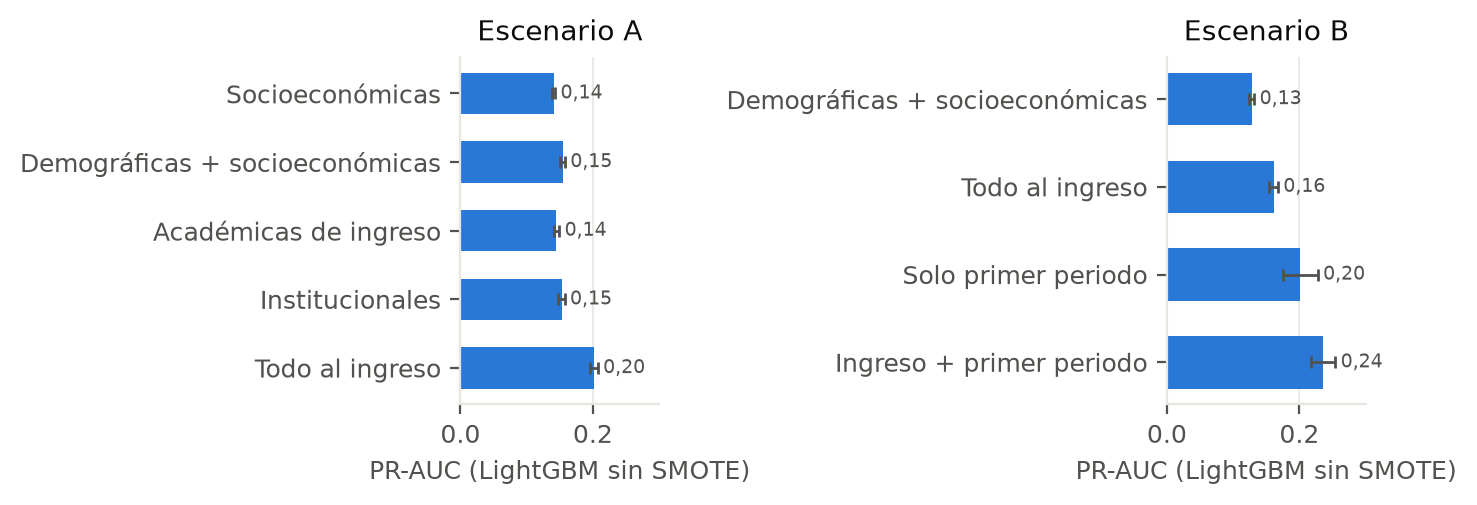
\includegraphics[width=0.86\linewidth]{fig06_ablacion.png}
\caption{PR-AUC de LightGBM según el grupo de variables usado (promedio de cinco rondas; las barras indican la desviación estándar).}
\label{fig:ablacion}
\end{figure}

\textbf{Variables más influyentes.} SHAP asigna a cada variable su contribución a la predicción de cada estudiante. Se aplicó a CatBoost nativo en ambos escenarios, porque es el mejor en el A, no se distingue del mejor en el B y, al no usar SMOTE, sus explicaciones no dependen de datos sintéticos. El cálculo se repitió en las cinco rondas para verificar que las conclusiones fueran estables (Figura~\ref{fig:shap}). Al ingreso, las variables más influyentes son la nota de matemáticas de admisión, la región del campus, el promedio de bachillerato y el porcentaje de beca, que ocupan los cuatro primeros lugares en todas las rondas. Al terminar el primer semestre, el promedio de ese semestre es la variable más importante en todas las rondas, con el doble de peso que la siguiente (porcentaje de beca). Su efecto no es lineal: un promedio bajo eleva mucho el riesgo, mientras que un promedio alto lo reduce poco. En ambos escenarios, las becas más altas y un mejor desempeño previo se asocian con menor riesgo. Estas relaciones son predictivas, no causales.

\begin{figure}[H]
\centering
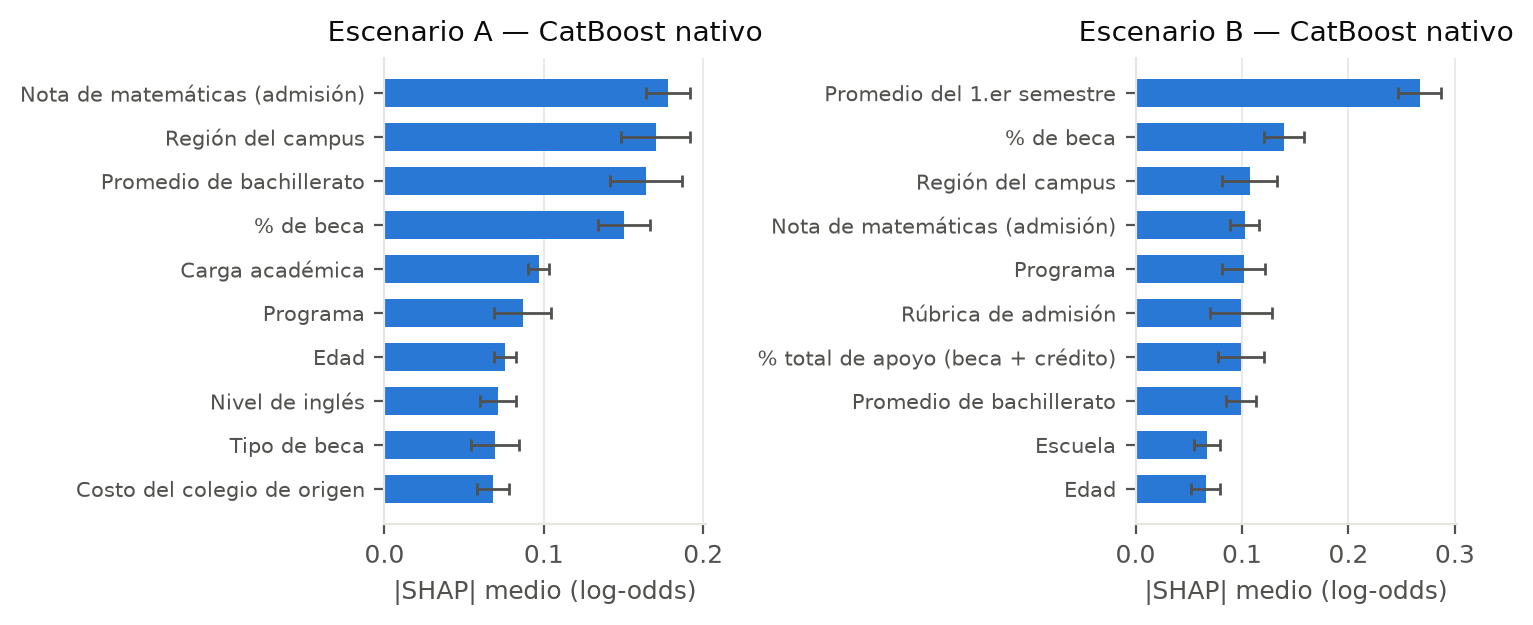
\includegraphics[width=0.86\linewidth]{fig07_shap_importancia.png}
\caption{Importancia de cada variable según SHAP (promedio de cinco rondas; las barras indican la desviación estándar entre rondas).}
\label{fig:shap}
\end{figure}

\textbf{Errores e implicaciones.} El modelo casi no detecta a los desertores que tienen beca por talento académico (detecta entre 6 y 11 de cada 100): su riesgo es bajo y las razones por las que se van no aparecen en los datos. En cambio, emite alertas para cerca del 65\,\% de los estudiantes sin beca que no desertan. Por ello, el modelo debe usarse para priorizar el acompañamiento y no para etiquetar a los estudiantes, ya que varias de sus señales reflejan condiciones socioeconómicas.

\textbf{Pasos para la entrega final.} Evaluar el modelo elegido en el conjunto de prueba, ampliar las rejillas señaladas en la Sección~3 y desplegar el modelo en una aplicación de Streamlit que explique cada predicción.

\textbf{Declaración de uso de IA generativa.} Se utilizó un asistente de inteligencia artificial (Claude, de Anthropic) como apoyo en la escritura del código y la revisión del texto. Los autores verificaron los resultados y pueden sustentar cada decisión técnica.

% ================= BIBLIOGRAFÍA =================
\begin{thebibliography}{9}
\footnotesize
\setlength{\itemsep}{1pt}

\bibitem{villar2024}
Villar, A. \& Robledo Velini de Andrade, C. (2024). Supervised machine learning algorithms for predicting student dropout and academic success: a comparative study. \textit{Discover Artificial Intelligence}, 4:2. \url{https://doi.org/10.1007/s44163-023-00079-z}

\bibitem{alvarado2022}
Alvarado-Uribe, J., Mejía-Almada, P., Masetto Herrera, A. L., Molontay, R., Hilliger, I., Hegde, V., Montemayor Gallegos, J. E., Ramírez Díaz, R. A., \& Ceballos, H. G. (2022). Student Dataset from Tecnologico de Monterrey in Mexico to Predict Dropout in Higher Education. \textit{Data}, 7(9), 119. \url{https://doi.org/10.3390/data7090119}

\bibitem{martins2021}
Martins, M. V., Tolledo, D., Machado, J., Baptista, L. M., \& Realinho, V. (2021). Early prediction of student's performance in higher education: a case study. En \textit{Trends and Applications in Information Systems and Technologies}, vol. 9 (pp. 166--175). Springer.

\bibitem{nadeau2003}
Nadeau, C. \& Bengio, Y. (2003). Inference for the generalization error. \textit{Machine Learning}, 52(3), 239--281.

\bibitem{chawla2002}
Chawla, N. V., Bowyer, K. W., Hall, L. O., \& Kegelmeyer, W. P. (2002). SMOTE: synthetic minority over-sampling technique. \textit{Journal of Artificial Intelligence Research}, 16, 321--357.

\bibitem{lundberg2017}
Lundberg, S. M. \& Lee, S.-I. (2017). A unified approach to interpreting model predictions. \textit{Advances in Neural Information Processing Systems}, 30.

\end{thebibliography}

\end{document}
